\documentclass[letterpaper, 10pt, DIV=13]{scrartcl}
\usepackage[T1]{fontenc}
\usepackage[english]{babel}
\usepackage{amsmath, amsfonts, amsthm, xfrac}
\usepackage{listings}
\usepackage{color}
\usepackage{longtable}
\usepackage{etaremune}

\numberwithin{equation}{section}
\numberwithin{figure}{section}
\numberwithin{table}{section}

\usepackage{sectsty}
\allsectionsfont{\normalfont\scshape} % Make all section titles in default font and small caps.

\usepackage{fancyhdr} % Custom headers and footers
\pagestyle{fancyplain} % Makes all pages in the document conform to the custom headers and footers

\fancyhead{} % No page header - if you want one, create it in the same way as the footers below
\fancyfoot[L]{} % Empty left footer
\fancyfoot[C]{} % Empty center footer
\fancyfoot[R]{\thepage} % Page numbering for right footer

\renewcommand{\headrulewidth}{0pt} % Remove header underlines
\renewcommand{\footrulewidth}{0pt} % Remove footer underlines
\setlength{\headheight}{13.6pt} % Customize the height of the header

\lstset{numbers=left, numberstyle=\tiny, stepnumber=1, numbersep=5pt}

% Colors and lstset for syntax highlighting from https://www.overleaf.com/latex/examples/syntax-highlighting-in-latex-with-the-listings-package/jxnppmxxvsvk
\definecolor{mygreen}{rgb}{0,0.6,0}
\definecolor{mygray}{rgb}{0.5,0.5,0.5}
\definecolor{mymauve}{rgb}{0.58,0,0.82}
\lstset{
  backgroundcolor=\color{white},   % choose the background color
  basicstyle=\footnotesize,        % size of fonts used for the code
  breaklines=true,                 % automatic line breaking only at whitespace
  captionpos=b,                    % sets the caption-position to bottom
  commentstyle=\color{mygreen},    % comment style
  escapeinside={\%*}{*},          % if you want to add LaTeX within your code
  keywordstyle=\color{blue},       % keyword style
  stringstyle=\color{mymauve},     % string literal style
}

\setlength\parindent{0pt}
\pagenumbering{gobble}

\title {
	\normalfont
	\huge{Rust-eze} \\
	\vspace{10pt}
	\large{CMPT 331 - Spring 2023 | Dr. Labouseur}
}

\author{\normalfont Josh Seligman | joshua.seligman1@marist.edu}
\date{\normalfont May 10, 2023}

\pagenumbering{arabic}
\begin{document}
\maketitle
\newpage

\section{Introduction}
Rust-eze is modern, object-oriented, type-safe programming language. It inherits
the best parts of Rust and Java to provide a fast and memory-safe languge for
the object-oriented paradim, while also bringing in some influence from Pascal.
Rust-eze does, however, differ from its parent languages in the following ways:
\begin{enumerate}
    \item Rust-eze is an object-oriented language, which means there are no
          structs and only classes/objects and enums.
    \item Like Java, but unlike Rust, Rust-eze is statically typed, so all
          variables must be explicitly defined with their respective types.
    \item Similar to Rust, but unlike Java, Rust-eze uses a system of borrowing
          and ownership so only one variable can point to a given place in
          memory at a time. This prevents the need for a garbage collector as
          variables are automatically dropped and the memory is freed when they
          go out of scope.
    \item Unlike Java, but like Rust, Rust-eze is compiled into the native
          binary, so there is no need for a JVM or an intermediate bytecode
          representation of Rust-eze programs.
    \item Similar to Rust, all instance variables must be initialized within the
          constructor.
    \item Similar to both parent languages, all classes belong to a module
          (Java package). However, more similar to Rust, the module is inferred
          based on the relative file location and does not have to be explicitly
          defined within the file.
\end{enumerate}

\newpage

\subsection{Genealogy}
\begin{figure}[ht]
    \centering
    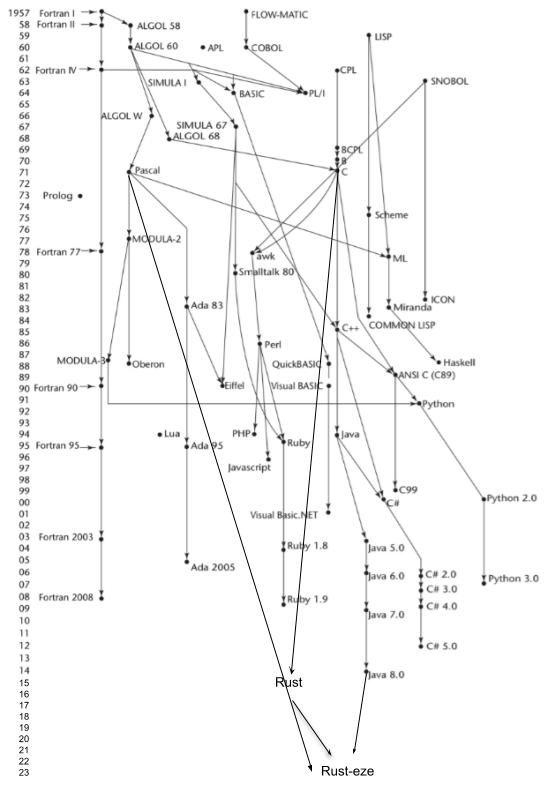
\includegraphics[height=6.5in]{genealogy}
\end{figure}

\newpage

\subsection{Hello World}
\begin{lstlisting}[caption = HelloWorld.rez, frame = single, nolol]
model HelloWorld
start
    pub fn main(Vec<String> args)
    start
        println("Hello world!");
    finish main
finish HelloWorld
\end{lstlisting}

\subsection{Program Structure}
The key organizational concepts in Rust-eze are as follows:
\begin{enumerate}
    \item Every file contains a single \textbf{model} (equivalent to a class),
          which should be the same name as the file minus the \textit{.rez} file
          extension.
    \item All instance members are by default private unless they are declared
          with the \textbf{pub} keyword.
    \item Instance variables are declared within the \textbf{specs} block and
          must be initialized within the constructor, which is a function that
          is the same name as the model.
    \item Local variables are immutable by default unless they are declared with
          the \textbf{mut} keyword.
    \item The entry point for all Rust-eze programs is the main method that is
          located in one of the models of the project.
\end{enumerate}

The program below defines a new \textbf{model} called Lightning that contains
3 instance variables: a String that is public called \textit{name}, a public
integer called \textit{age}, and a private integer called \textit{miles}. Each
of these instance variables are initialized within the constructor. Each
Lightning has 2 member functions: \textit{drive} and \textit{say\_it}.
\textit{drive} is a public method as it is defined with the \textbf{pub}
keyword. Since it modifies an instance variable, it must take it a mutable
reference to the object in addition to the number of miles being driven. Inside
of the method, a new local variable called \textit{new\_mileage} is declared
without the \textbf{mut} keyword, meaning that it is immutable and is a constant
with the value it is initialized with. The other instance method,
\textit{say\_it}, is also public and does not modify the instance variables,
which is why it needs an immutable reference to \textbf{self}.

\begin{lstlisting}[caption = Lightning.rez, frame = single, nolol]
model Lightning
start
    specs
    start
        pub String name;
        pub int age;
        int miles;
    finish specs

    pub fn Lightning(String my_name, int my_age)
    start
        self.name := my_name;
        self.age := my_age;
        self.miles := 0;
    finish Lightning

    pub fn drive(&mut self, int num_miles)
    start
        int new_mileage := self.miles + num_miles;
        self.miles := new_mileage;
    finish drive

    pub fn say_it(&self)
    start
        println("Kachow!");
    finish say_it
finish Lightning
\end{lstlisting}

Next, the Lightning model is imported to a new file called \textit{Main.rez}
and is initialized within the main method. Since the \textbf{mut} keyword is
used, we can use the mutable method of \textit{drive} on the new object as well
as directly modify its public instance variables. After \textit{the\_lightning}'s
name is printed, we call its \textit{say\_it} method and then call the
\textit{drive} method with an input of 42 miles to increase the object's mileage.

\begin{lstlisting}[caption = Main.rez, frame = single, nolol]
import garage.Lightning;

model Main
start
    pub fn main(Vec<String> args)
    start
        mut Lightning the_lightning := new Lightning("McQueen", 17);
        println(the_lightning.name);

        the_lightning.say_it();
        the_lightning.drive(42);
    finish main
finish Main
\end{lstlisting}

\subsection{Types and Variables}
There are two kinds of variables in Rust-eze: \textbf{\textit{value types}} and
\textbf{\textit{reference types}}. Variables of value types directly contain
their data, while variables of reference types store references to their data or
objects in memory. Due to the ownership system, only one variable of a reference
type can point to a particular place in memory at a given time. See Section 3
for details.

\subsection{Visibility}
In Rust-eze, visibility of methods and instance variables is defined as either
public or private. Everything is default private unless explicitly stated to be
public. Once a variable or method is public, it may be accessed outside of the
model in which it is defined.

\subsection{Statements Differing from Rust and Java}
\begin{center}
\begin{longtable}{|p{2in}|p{4in}|}
\hline
\textbf{Statement} & \textbf{Example} \\
\hline
Assignment statement & \begin{lstlisting}[nolol, numbers = none]
mut int x := 5;
x = 3;
int y := x + 2;
\end{lstlisting} \\
\hline
If statement & \begin{lstlisting}[nolol, numbers = none]
int x := 7;
if x > 3 && x < 9
start
    println("Hello there")
else
    println("Kachow")
finish if
\end{lstlisting} \\
\hline
\hline
For loop & \begin{lstlisting}[nolol, numbers = none]
for (mut int i in range(0, 10, 1))
start
    println(i)
finish for
\end{lstlisting} \\
\hline
\end{longtable}
\end{center}

\section{Lexical Structure}
\subsection{Programs}
A Rust-eze program consists of one or more source files. A source file is an
ordered sequence of (probably) Unicode characters. 
\\ \\
Conceptually speaking, a program is compiled using five steps:
\begin{enumerate}
    \item Transformation, which converts a file from a particular character
          repertoire and encoding scheme into a sequence of Unicode characters.
    \item Lexical analysis, which translates a stream of Unicode input
          characters into a stream of tokens.
    \item Syntactic analysis (parsing), which translates the stream of tokens
          into a concrete syntax tree (CST).
    \item Semantic analysis, which converts the CST into an abstract syntax tree
          (AST) and is passed to the semantic analyzer for type checking and the 
          borrow checker to make sure all variables referenced are active owners
          of data.
    \item Code generation, which converts the AST into executable code for the
          target platform and CPU architecture.
\end{enumerate}
\subsection{Grammars}
This specification presents the syntax of the Rust-eze programming language
where it differs from Rust and Java.
\subsubsection{Lexical grammar (tokens) where different from Rust and Java}
<assignment operator> $\rightarrow$ := \\
<block begin> $\rightarrow$ start \\
<block end> $\rightarrow$ finish \\
<print> $\rightarrow$ println \\
<visibility modifier> $\rightarrow$ pub | $\epsilon$ \\
<mutability modifier> $\rightarrow$ mut | $\epsilon$ \\

\subsubsection{Syntactic ("parse") grammar where different from Rust and Java}
<model definition> $\rightarrow$ model <model name> <block begin> <statements>
                                 <block end> <model name> \\
<specs definition> $\rightarrow$ specs <block begin> <spec definition> <block end> \\
<spec definition> $\rightarrow$ <visibility modifier> <type> <spec name>;
                                <spec definition> | $\epsilon$ \\
<variable declaration> $\rightarrow$ <mutability modifier> <type> <variable name>
                                     <assignment operator> <epression>; \\
<for loop> $\rightarrow$ for (mut <type> <var name> in <expr>) <block begin>
                         <statements> <block end>

\subsection{Lexical Analysis}
\subsubsection{Comments}
Rust-eze supports two forms of comments: single-line and multi-line comments.
Single-line comments start with the characters // and extend to the end of the
line in the source file. Multi-line comments begin with /* and end with */ and
may span multiple lines. Comments do not nest.

\subsection{Tokens}
There are several kinds of tokens: identifiers, keywords, literals, operators, 
and punctuators. White space and comments are not tokens, though they act as
separators for tokens where needed. \\
Tokens:
\begin{itemize}
    \item identifier
    \item keyword
    \item integer literal
    \item real literal
    \item character literal
    \item string literal
    \item operator or punctuator
\end{itemize}

\subsubsection{Keywords Different from Rust and Java}
\textbf{New keywords:} range, model, specs, start, finish \\
\textbf{Removed keywords:} use, class, match, do, private, byte, short, str,
                           boolean, static, public, void, i32, float \\

\section{Type System}

\subsection{Type Rules}

\subsection{Value Types (Different from Rust and Java)}

\subsection{Reference Types (Different from Rust and Java)}

\section{Example Programs}
\subsection{Caesar Cipher Encrypt}

\subsection{Caesar Cipher Decrypt}

\subsection{Factorial}

\subsection{Sort}

\subsection{Program 1}

\subsection{Program 2}

\end{document}
